\subsection{Infrared}
\subsubsection{Luminosity Function}
When analysing the \gls{lf} of IR galaxies, it is paramount that both the SF and AGN LF are analysed in parallel. Otherwise, crucial information regarding the underlying physical co-evolution between the processes will be omitted, and incorrect individual conclusions will be drawn. As was reviewed in \cref{Sec: Feedback}, \gls{ir} emission probes both \gls{sf} and \gls{agn} activity \citep{fu_decomposing_2010}. The literature contains limited research on \gls{agn} \gls{lf}s and even less on \gls{ir} \gls{agn} \gls{lf}. Consequently, the \gls{ir} \gls{agn} \gls{lf} represents a relatively unexplored approach to quantifying the co-evolution of galaxies and BHs. Most authors have concentrated on the galaxy or \gls{sf} \gls{lf}, which traces the evolution of galaxies \citep{cool_galaxy_2012, tempel_tracing_2011}. However, these studies often overlook the co-evolution with BHs \citep{fotopoulou_5-10_2016, symeonidis_agn_2021, finkelstein_coevolution_2022} that galaxies have been shown to depend on \citep{hopkins_cosmological_2008, fiore_agn_2017}.

One of the most commonly used methods for calculating \gls{lf} is with the Schechter function \citep{schechter_analytic_1976}. However, \cite{wu_mid-infrared_2011} reports that the mid-\gls{ir} wavelengths exhibit a shallower exponential profile inconsistent with a Schechter function. According to \cite{fu_decomposing_2010}, this discrepancy may be attributed to \gls{agn} contamination of the \gls{lf} and, when removed, can accurately describe a Schechter function. Indeed, this is the case for IR \gls{agn} \gls{lf}s, which are inconsistent with a Schechter function \citep{symeonidis_what_2019}. The Saunders function \citep{saunders_60-mum_1990} is typically used to model \gls{agn} \gls{lf}s. 

The properties of IR light make it the ideal regime for studying heavily obscured (Type 2) \gls{agn}. Type 2 sources absorb most of the outgoing X-ray, Optical, and UV wavelengths and re-emit their radiation in the IR domain \citep{fu_decomposing_2010, wu_mid-infrared_2011, gruppioni_modelling_2011, assef_mid-ir-_2011, toba_9_2013, oconnor_luminosity_2016, brown_infrared_2019, symeonidis_agn_2021}. The ability to detect both types of \gls{agn} significantly influences the decision to study IR \gls{lf}s, as other wavelengths struggle to identify heavily obscured sources. However, as noted by \cite{katsianis_evolution_2017}, infrared observations are primarily practical for dusty, massive galaxies and become limited at higher redshifts. Additionally, less obscured (Type 1) \gls{agn} may appear dimmer in the IR because they emit less light from reprocessing other wavelengths around the dusty torus. 

Results by \cite{han_evolution_2012} show the faint end slope of the \gls{lf} flattens with increasing redshift. However, this may be due to poor sampling of the faint end, which could be a binning effect or Malmquist bias, as discussed previously \citep{madau_cosmic_2014}. Splitting the \gls{lf} into redshift and luminosity bins reduces sample sizes, leading to an increase in errors and error propagation \citep{dai_mid-infrared_2009}. However, it is also necessary because it allows evolution to be studied across cosmic time \citep{wu_mid-infrared_2011, wylezalek_galaxy_2014}. It remains possible that surveys designed to probe fainter luminosities at greater redshift will uncover many smaller ``building block-style" dwarf galaxies as current leading theories of cosmology and \gls{lss} predict \citep{magorrian_demography_1998, ziparo_primordial_2024}. Although, as was reviewed in \cref{Sec: First Stars}, results by \cite{labbe_population_2023} have cast doubt on these theories.

The goal of this thesis is to utilise the decomposed \gls{agn} and \gls{sf} emission to generate and analyse the simultaneous evolution of the \gls{agn} and \gls{sf} \gls{lf}. By performing this analysis, we can place constraints on the co-evolution of galaxies and their central BHs. This work is significant because it is a relatively unexplored avenue; the decomposed IR AGN LF has only been explored a handful of times in the past \citep{valiante_backward_2009, fu_decomposing_2010, gruppioni_modelling_2011}. With the advent of new \gls{sed} codes like \texttt{CIGALE} \citep{boquien_cigale_2019}, new and exciting results concerning galaxy and \gls{agn} co-evolution are to be discovered.

\subsubsection{Parameter Evolution}

\begin{figure}[ht!]
    \centering
    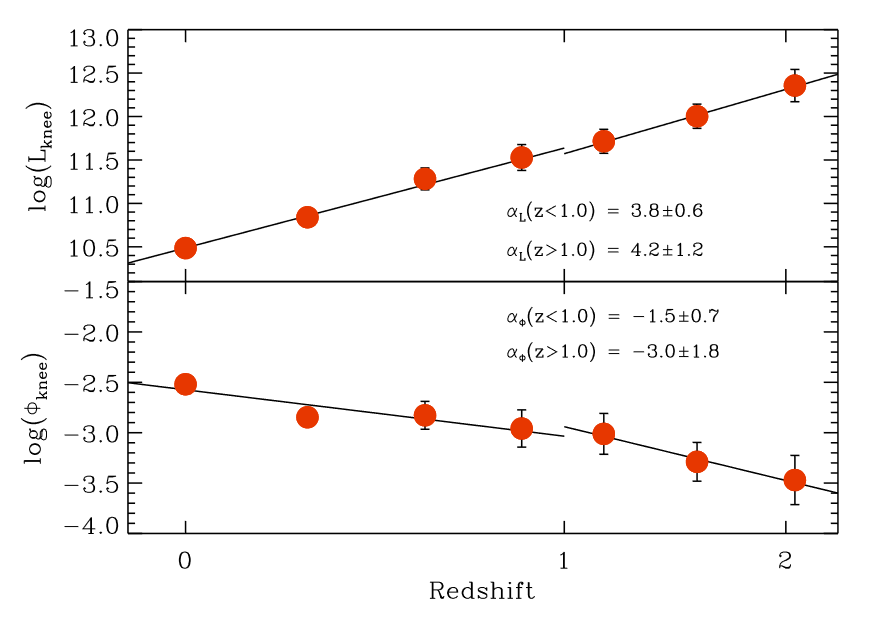
\includegraphics[width=0.95\linewidth]{Figures/magnelli_param.png}
    \caption{Evolution of free fitting parameters to the LF from \cite{magnelli_deepest_2013}. Top: evolution of $L^*$. Bottom: evolution of $\phi^*$. The evolution of both parameters is fit twice with a break at $z=1$. The parameters evolve differently at $z>1$ than $z<1$. Credit: B. Magnelli, 553, A132, 17, 2013, reproduced with permission © ESO.}
    \label{Fig: Example Magnelli Param}
\end{figure}

The Schechter \citep{schechter_analytic_1976} and Saunders \citep{saunders_60-mum_1990} functions evolve with redshift. Both functions use a power-law decline at the faint-end, $\alpha$, but the Saunders function incorporates an additional Gaussian bright-end slope, $\sigma$. Both functions also use two free-fitting parameters, $L^{*}$ and $\phi^{*}$, representing the characteristic luminosity and density, respectively. This allows for the characterisation of intrinsic properties in various populations of galaxies. \Cref{Fig: Example Magnelli Param} displays an example figure of the evolution of the free fitting parameters by \cite{magnelli_deepest_2013}. The characteristic luminosity, $L^{*}$, represents the average luminosity at the ``knee" of the \gls{lf}. The characteristic density, $\phi^{*}$, again represents the average density at the ``knee" of the \gls{lf} in each redshift bin.

A problem in the process of fitting the free parameters, $L^{*}$ and $\phi^{*}$, is the degeneracy between the two. Many authors have trouble decisively fitting the free parameters to fit best the observed shape of the \gls{lf} \citep{caputi_infrared_2007, hopkins_observational_2007, rodighiero_mid-_2010, casey_redshift_2012, gruppioni_herschel_2013, shen_bolometric_2020}. Instead of using the best-fit values to derive meaning, the observed trend in the redshift evolution is often utilised. The evolution of the free parameters is broadly consistent across the literature: $L^{*}$ is positively correlated with redshift, and $\phi^{*}$ is negatively correlated with redshift. However, \cite{delvecchio_tracing_2014} finds \gls{agn} $\phi^{*}$ reaches a peak at $z=0.5$ and declines toward $z=0$. This suggests that a significant evolutionary epoch occurs below $z<1$, possibly due to AGN feedback in the local universe suggested by \cite{katsianis_evolution_2017}. Furthermore, \cite{delvecchio_tracing_2014} does not find a corresponding increase in $L^{*}$ evolution at the same time as the peak of $\phi^{*}$, suggesting that the quenching process in the local universe may be accelerated by \gls{agn} feedback \citep{silk_unleashing_2013, fiore_agn_2017}. No peak in the evolution of the \gls{sf} $L^{*}$ occurs at $z=2$ to coincide with the peak of cosmic \gls{sf} history because the peak is driven by both $L^{*}$ and $\phi^{*}$ \citep{assef_mid-ir-_2011, wu_mid-infrared_2011}.

\subsubsection{Luminosity Density}
The luminosity density ($\rho_{IR}$) is obtained by integrating under the best-fitting luminosity function. This is also known as the Star Formation Rate Density (SFRD) for stars (through which the famous peak at $z=2$ is observed --- \citealp{madau_cosmic_2014}) and Black Hole Accretion Rate Density (BHARD) for AGN. This is then converted into a \gls{sfr} using the \cite{kennicutt_global_1998} relation and measured in $M_\odot \ yr^{-1} \ Mpc^{-1}$. The SFRD is well known, cited thousands of times and appears in as many works. \Cref{Fig: Example Traina Luminosity Density} shows the \gls{sfr} density of some of the most cited works combined by \cite{traina_a3cosmos_2024}.

\begin{figure}[ht]
    \centering
    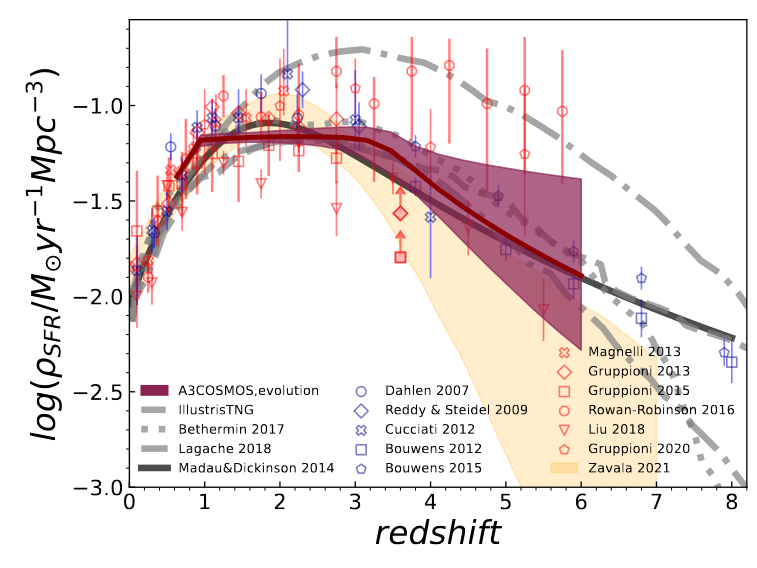
\includegraphics[width=\linewidth]{Figures/traina_LD.png}
    \caption{Evolution of the cosmic SFR density of the most prominent works combined by \cite{traina_a3cosmos_2024}. Every author finds the peak occurring at $z=2$. Differences between findings grow mostly beyond $z>2.5$. The SFR grew from when the universe was only a few hundred Myrs old before reaching the peak when the universe was only 3.3 Gyrs old. SFR has been declining for over 10 Gyrs.}
    \label{Fig: Example Traina Luminosity Density}
\end{figure}

Comparatively, little is known about the AGN density \citep{delvecchio_tracing_2014}, although the \gls{agn} density has been observed approximately one order of magnitude below the SFRD \citep{delvecchio_tracing_2014, symeonidis_agn_2021}. An observed offset in the peak densities would provide invaluable clues to the co-evolution of \gls{agn} and \gls{sf}. It is difficult to speculate what such an offset would mean for the overall co-evolution because the complex interactions between galaxies and \gls{agn} have positive and negative influences under various circumstances. A peak in the AGN density at any redshift has not yet been sufficiently narrowed, existing between $1<z<3$, highlighting the importance of pushing observations towards higher redshifts with greater sensitivity (see \citealp{delvecchio_tracing_2014, symeonidis_agn_2021} for examples). This thesis aims to contribute significantly to this active area of research. Future studies should explore this more deeply to obtain a complete picture of the co-evolution of \gls{sf} and \gls{agn}.

\begin{figure}[ht!]
    \centering
    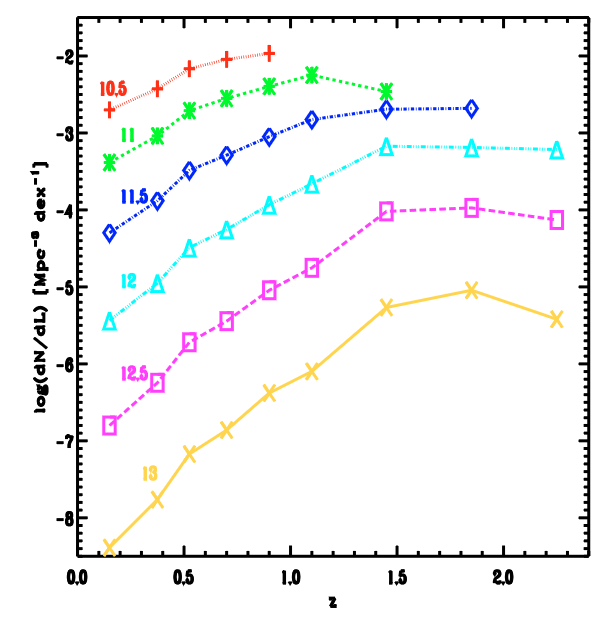
\includegraphics[width=\linewidth]{Figures/rodig_CE.png}
    \caption{The redshift evolution of the space density of various luminosity classes recreated from \cite{rodighiero_mid-_2010}. It can be readily identified that the most luminous galaxies decline in number density earlier and more rapidly than their fainter luminosity counterparts, also known as the downsizing effect. Fainter luminosities and higher redshifts are required to measure the effect precisely. Credit: G. Rodighiero, A\&A,  515, A8, 19, 2010, reproduced with permission © ESO.}
    \label{Fig: Example Rodighiero Class Evolution}
\end{figure}

\subsubsection{Class Evolution} \label{Sec: Intro Downsizing}
The evolution of different luminosity classes with redshift can be directly derived from the changes in the \gls{lf}. \cite{han_evolution_2012} observed a \textit{downsizing} effect in their study of \gls{agn}, indicating the number density of bright AGN peaks at higher redshift compared to fainter AGN. Moreover, \cite{merloni_synthesis_2008} found a reversal in the downsizing effect above $z=2$, coinciding with the peak of cosmic \gls{sfr} density. These results are displayed in \Cref{Fig: Example Rodighiero Class Evolution} by \cite{rodighiero_mid-_2010}. 

The implications of a downsizing effect are profound: galaxies in the earlier universe became more abundant until $z\approx2$ when the brightest began to decline. \cite{fiore_agn_2017} speculates that the downsizing effect may originate from feedback mechanisms. The various types of feedback reviewed in \cref{Sec: Feedback} all have the potential to either positively or negatively influence the downsizing of both \gls{sf} and \gls{agn}. Future work is needed in this area to provide a more complete understanding. It remains unclear whether the downsizing effects in \gls{sf} and \gls{agn} are fundamentally different or if they affect each other. Results by \cite{fanidakis_evolution_2012} suggest that the largest galaxies consume their gas supply faster than their less-massive counterparts, leading to quiescence sooner and more rapidly. Importantly, the ``building block" theory of \gls{lss} still holds, supporting \cite{fanidakis_evolution_2012} results \citep{magorrian_demography_1998}.

\subsubsection{Conclusions}
A wealth of avenues exists to analyse the evolution of the \gls{lf}. Both \gls{sf} and \gls{agn} variations can be independently examined simultaneously to uncover unique perspectives on galaxy evolution and \gls{agn} co-evolution. The free parameters' evolution will allow us to analyse how the \gls{lf} is evolving over time. The luminosity density can deduce information about the activity of \gls{sf} and \gls{agn} throughout the universe's history. The evolution of various luminosity classes can reveal how different sizes and luminosities of objects have evolved over cosmic time. In this thesis, we will utilise all these probes to comprehensively understand galaxy evolution and \gls{agn} co-evolution. 

% For example, AGN density peaking before \gls{sf} may indicate \gls{agn} have a positive influence on their host galaxy, but a later peak may suggest a negative influence on \gls{sfr}. \textcolor{red}{cowley 2018?}

% The unified \gls{agn} model states there are two types of \gls{agn} \cite{toba_9_2013}. Type 1 \gls{agn}s are characterised by the presence of broad emission lines in their spectra and show an unobstructed view along a direct line of sight to the centre. Type 2 \gls{agn}s, on the other hand, exhibit only narrow emission lines in their spectra and are associated with an obscured line of sight to the centre. A direct view of the broad-line region is blocked or heavily absorbed by intervening material, such as the dusty torus. As a result, X-ray and UV wavelengths are utilised (cite) but omit the vast majority of Type 2 \gls{agn} galaxies from their analysis. This is a major factor influencing the decision to study IR \gls{lf}s as IR can detect both Types of \gls{agn} whereas other wavelengths cannot, or at best, struggle greatly. Furthermore, the dusty torus surrounding the black hole absorbs most of the outgoing optical, UV, and X-ray radiation that is subsequently re-emitted in the IR regime \citep{fu_decomposing_2010, assef_mid-ir-_2011, wu_mid-infrared_2011, han_evolution_2012, toba_9_2013, brown_infrared_2019, symeonidis_agn_2021}, again highlighting the usefulness of IR light over other wavelengths. Some research exists that challenges the unified \gls{agn} model and suggests the reality of \gls{agn} obscuration is far more complex than simple viewing angles might have us believe. \cite{han_evolution_2012} concluded that the obscuration resulting from the dusty torus must evolve over time. Indeed, \cite{brown_infrared_2019} agrees, finding that the line of sight towards \gls{agn}s is not the deciding factor on the resulting \gls{agn} type. The consequence of this ambiguity between whether different \gls{agn} types even exist means it is important to keep one consolidated \gls{agn} IR \gls{lf} instead of separating into two isolated \gls{lf}s, one for each type respectively.

% The Schechter function is particularly useful for describing the luminosity function of galaxies because it captures the observed features, such as a power-law decline at the faint end and an exponential cutoff at the bright end. Yet, there is a dilemma: \cite{wu_mid-infrared_2011} reports that the UV and optical wavelengths follow a Schechter function, but the IR wavelengths have a shallower exponential inconsistent with a Schechter function. \cite{fu_decomposing_2010} proposes that this is due to \gls{agn} contribution to the \gls{lf}, and when removed, can fit a Schechter function normally. Indeed, there is much agreement in the literature that the observed IR light contains both SF and \gls{agn} components (cite). Interestingly, though, few sources separate the SF and \gls{agn} light (cite), mostly because, until recently, this was very difficult to accomplish accurately (cite).

% The ZFOURGE survey offers a unique advantage by investigating galaxies at higher redshifts and fainter luminosities, leading to a deeper understanding of galaxy-BH co-evolution through discoveries at lower luminosities \citep{straatman_fourstar_2016}. By combining ZFOURGE data with \gls{lf}s, more powerful constraints can be placed on galaxy-BH co-evolution.

% For example, the activity of \gls{agn} suppressing \gls{sf} \citep{fanidakis_evolution_2012}, or supernova feedback potentially suppressing or even aiding \gls{sf} as well \citep{sokasian_cosmic_2004, klessen_first_2023}.  

% This is likely because the authors focus on the kinetic \gls{lf} of \gls{agn} jets and not \gls{agn} as a whole. Although \cite{fanidakis_evolution_2012} demonstrated clear downsizing of the entire \gls{agn}, which is irreconcilable with \cite{merloni_synthesis_2008}: how can there be more \gls{agn} jets than \gls{agn}? 

% \cite{wylezalek_galaxy_2014} proposes that the oldest stellar populations reside in massive clusters, the likes of which are not seen in the local universe \citep{croton_many_2006}. Intuitively, galaxy clusters likely support stronger \gls{sf}, but \cite{wang_imperial_2010} shows clusters are positively correlated with \gls{ir} luminosity, which \cite{symeonidis_agn_2021} indicated could be increasingly contaminated by \gls{agn}. Similarly, results from \cite{rodighiero_mid-_2010, gruppioni_herschel_2013} also revealed a \textit{downsizing} effect in \gls{sfg}s. 